\section[Rollende Kugel]{Gerader zentraler Stoß einer rollenden Kugel}



\begin{figure}[h!]
	\centering
	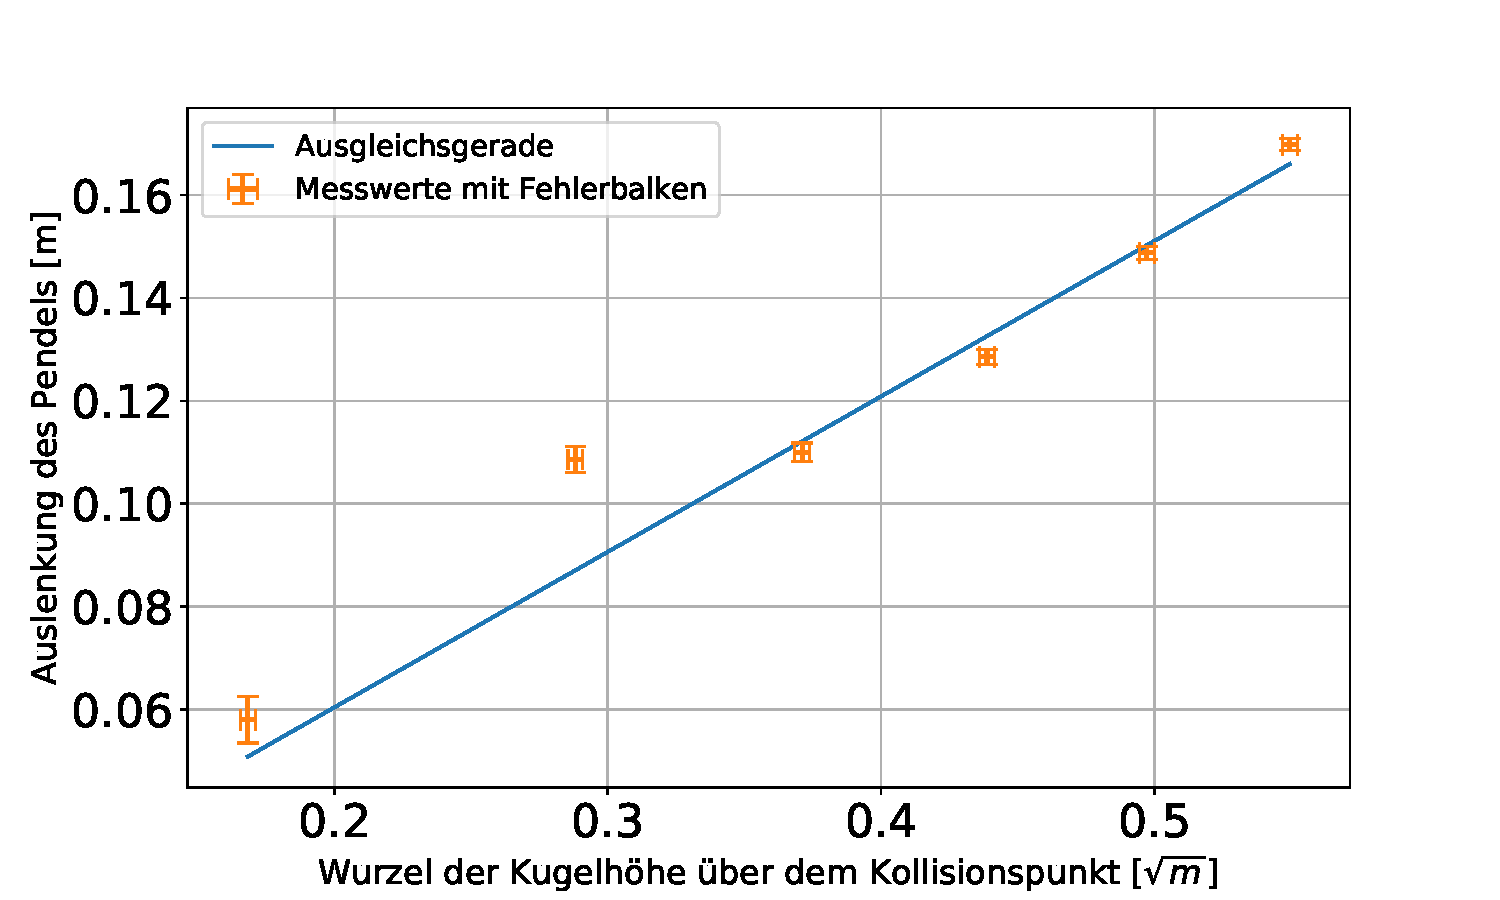
\includegraphics[width=0.7\linewidth]{res/Rinne}
	\caption{Ausschlag des Pendels in Abhängigkeit von $\sqrt{h}$}
	\label{fig:rinne}
\end{figure}

Die Auslenkung des Pendels in Abhängigkeit der Wurzel der Höhe $\sqrt{h}$ wurde in \cref{fig:rinne} dargestellt. Deutlich ist zu erkennen, dass der Messwert unterhalb von $\sqrt{h}=\SI{30}{\centi\metre}$ nicht zu der Geraden durch die anderen Messpunkte passt und nahezu identisch zu dem nächsthöheren Wert ist. Es wird daher davon ausgegangen, dass die Kugel an der falschen Markierung positioniert wurde und der Messpunkt wurde in der weiteren Auswertung ausgelassen.
\begin{table}
	\caption{Abmessungen des Versuchsaufbaus nach \cref{fig:rinneskizze} sowie des Pendels.}

\begin{tabular}{|l|c|}
	\hline 
	Höhe des Bahnendes über Stoßpunkt $h_0$ & \SI{30.20+-0.12}{cm}  \\ 
	\hline 
	Länge $L$ & \SI{0.5+-0.00012}{\metre}  \\ 
		\hline 
	Höhe $H$&  \SI{32.7+-0.12}{\centi \meter}\\ 
	\hline
	Masse der rollenden Kugel $m_1$& \SI{66.5 \pm 0.006}{\gram}  \\ 
	\hline 
	Masse des Pendels $m_2$ & \SI{0.51034+-0.000006}{\kilogram} \\  
	\hline
	Vertikale Länge des Pendels $l$ & \SI{1.737+-0.004}{\metre}  \\ 
	\hline 
\end{tabular} 
\label{tab:messwrinne}
\end{table}
Da die anderen Messwert auf einer Geraden durch den Ursprung liegen und die theoretischen Betrachtungen dies suggestiert wurden die Messpunkte an eine Funktion der Form $a(\sqrt{h})=b \sqrt{h}$ angepasst, man erhält $b=\SI{0.302+-0.004}{\sqrt{\metre}}$. Nach Gleichung \ref{eq:alenkrinne} und $b=\frac{a}{\sqrt{h}}$ erhalten wir:
\begin{align}
\varepsilon&=\left( \frac{(m_1+m_2)}{2m_1} \right) ^2 \cdot \frac{b^2}{2l}\\
\end{align}

Mit den Messwerten aus Tabelle \ref{tab:messwrinne} folgt $\varepsilon = 0.4943 \pm 0.0012$.














